\section{Results}
\label{sec:results}

\subsection{Trajectories}

\begin{table}[t]
\centering
\caption{Trajectories over training (mean of 3 seeds, 240 prompts each). Quality, preference, and flags are from \judgeone. ``Pref.'' is the probability that the judge prefers the checkpoint response over the step-0 response. The \rmodel score peaks at 60\% (bold) while judge quality and preference fall.}
\label{tab:traj}
\resizebox{\textwidth}{!}{
\begin{tabular}{@{}rccccccccc@{}}
\toprule
 & & \multicolumn{2}{c}{\judgeone} & \multicolumn{2}{c}{Surface} & \multicolumn{4}{c}{\judgeone flag rate} \\
\cmidrule(lr){3-4} \cmidrule(lr){5-6} \cmidrule(lr){7-10}
\% steps & \rmodel score & Quality & Pref. & Tokens & Hit cap & Verbosity & Sycophancy & Format & Fabrication \\
\midrule
0   & $-0.07$ & 5.52 & 0.500 & 215 & 0.19 & 0.685 & 0.029 & 0.033 & 0.214 \\
10  & 0.25 & {\bf 5.64} & 0.497 & 214 & 0.17 & 0.696 & 0.032 & 0.028 & 0.232 \\
20  & 0.61 & 5.62 & 0.490 & 237 & 0.21 & 0.757 & 0.032 & 0.033 & 0.249 \\
30  & 0.92 & 5.51 & 0.472 & 264 & 0.27 & 0.819 & 0.032 & 0.072 & 0.272 \\
40  & 0.99 & 5.30 & 0.433 & 267 & 0.28 & 0.839 & 0.031 & 0.076 & 0.290 \\
50  & 1.14 & 5.29 & 0.408 & 281 & 0.32 & 0.861 & 0.024 & 0.074 & 0.292 \\
60  & {\bf 1.21} & 5.12 & 0.376 & 290 & 0.38 & 0.850 & 0.022 & 0.092 & 0.319 \\
70  & 1.16 & 5.03 & 0.366 & 288 & 0.38 & 0.864 & 0.018 & 0.053 & 0.333 \\
80  & 1.15 & 4.85 & 0.351 & 294 & 0.42 & 0.853 & 0.017 & 0.058 & 0.381 \\
90  & 1.11 & 4.46 & 0.286 & 306 & 0.49 & 0.904 & 0.036 & 0.071 & 0.401 \\
100 & 0.96 & 4.50 & 0.302 & 285 & 0.41 & 0.840 & 0.021 & 0.046 & 0.422 \\
\bottomrule
\end{tabular}
}
\end{table}

\begin{figure}[t]
\centering
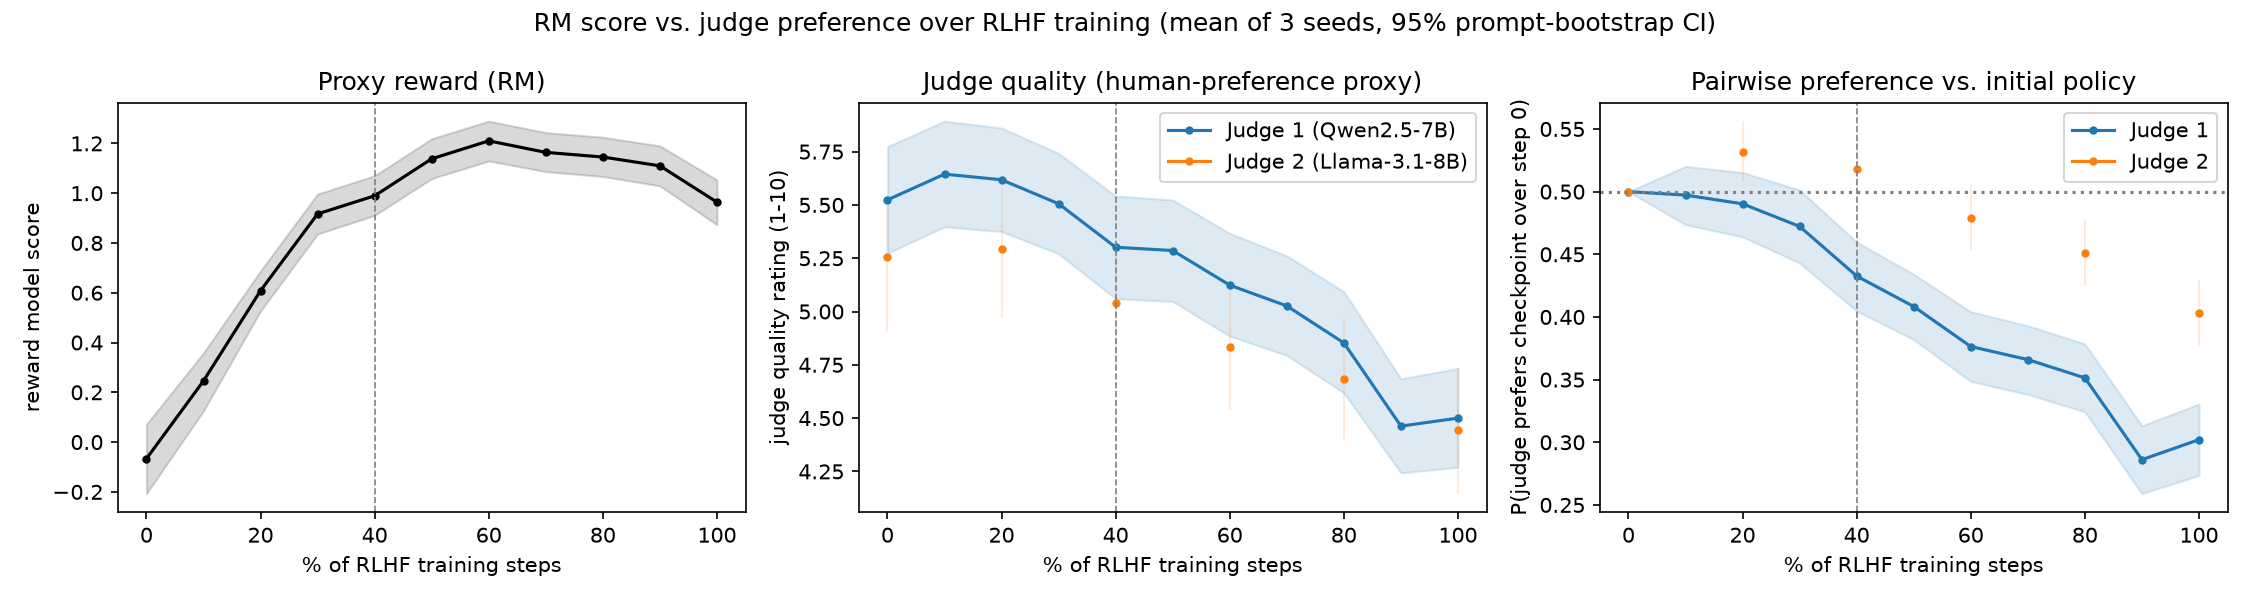
\includegraphics[width=0.98\linewidth]{figures/fig1_rm_vs_judge.png}
\caption{\rmodel score (left), judge quality rating (middle), and pairwise preference against the step-0 response (right) over training. Lines are means over 3 seeds with 95\% prompt-bootstrap intervals; \judgetwo is evaluated on a 20\% grid. The \rmodel score rises by about one standard deviation while both judges' quality ratings fall. The dashed line marks the 40\% checkpoint of H4.}
\label{fig:rm_vs_judge}
\end{figure}

\Tabref{tab:traj} and \figref{fig:rm_vs_judge} give the trajectories.
The \rmodel score rises from $-0.07$ to a peak of 1.21 at 60\% of training.
\rmodel scores have a standard deviation of about 1.3 across responses, so the peak gain is roughly one standard deviation.
Over the same period \judgeone's quality rating falls from 5.52 to 5.12, and it reaches 4.50 at the end.
Responses get longer (215 to 285 tokens) and the fraction that hit the 384-token cap doubles from 0.19 to 0.41.
Among the flags in \tabref{tab:traj}, verbosity and fabrication rise, format gaming rises and falls, and sycophancy stays flat at 2--4\%.

\subsection{H1: which categories make up reward-hacking instances?}

Of the 7,200 post-step-0 responses, 83.9\% have a higher \rmodel score than their step-0 counterpart, and 2,339 meet the full instance definition of \secref{sec:definitions}.

\begin{table}[t]
\centering
\caption{Primary-label shares among reward-hacking instances under the primary definition and four alternatives. \vsshare is verbosity plus sycophancy, with a 95\% prompt-bootstrap interval. H1 requires the lower bound to exceed 60\%; only the \judgetwo row does, and that row is uninformative because \judgetwo flags verbosity on 96.6\% of step-0 responses.}
\label{tab:shares}
\resizebox{\textwidth}{!}{
\begin{tabular}{@{}lrcccccc@{}}
\toprule
Instance definition & $n$ & Verbosity & Sycophancy & Fabrication & Evasion & Other & \vsshare share (95\% CI) \\
\midrule
Primary (\judgeone) & 2,339 & 49.3\% & 0.6\% & 34.5\% & 14.7\% & 0.9\% & {\bf 49.9\%} (45.3--54.3) \\
Alt A: judge rating lower than step 0 & 2,578 & 50.3\% & 0.7\% & 32.0\% & 16.5\% & 0.3\% & 51.0\% (46.2--55.9) \\
Alt B: \rmodel gain $>0.5$ SD & 1,514 & 48.1\% & 0.5\% & 39.2\% & 12.1\% & 0.2\% & 48.6\% (43.6--53.8) \\
Alt C: final checkpoint only & 308 & 47.1\% & 0.0\% & 39.3\% & 12.3\% & 1.3\% & 47.1\% (40.9--53.2) \\
\midrule
\judgetwo for instances and labels & 698 & 80.5\% & 0.3\% & 18.4\% & 0.9\% & 0.0\% & 80.7\% (76.3--84.9) \\
\bottomrule
\end{tabular}
}
\end{table}

\begin{figure}[t]
\centering
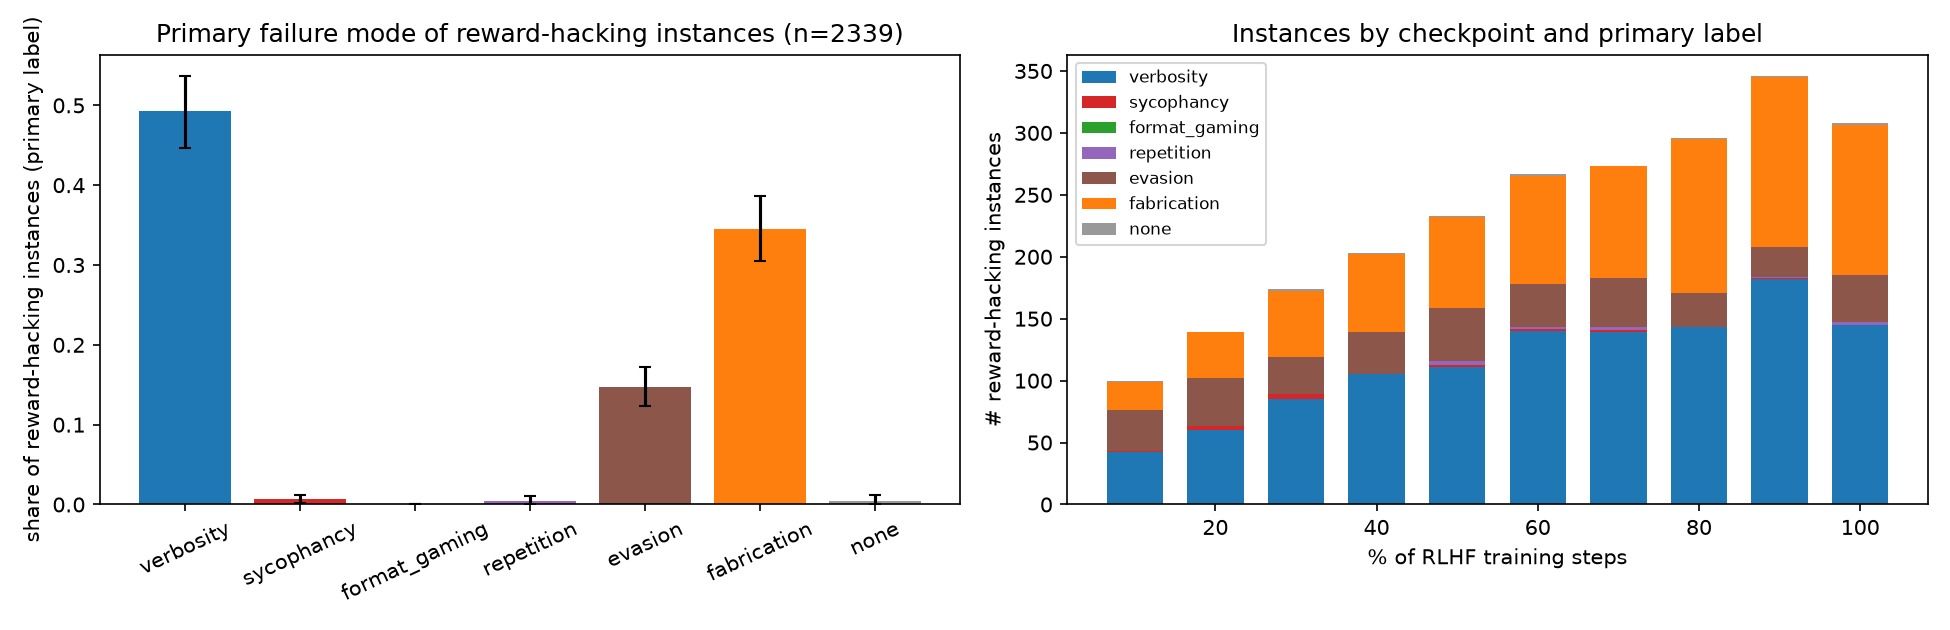
\includegraphics[width=0.98\linewidth]{figures/fig4_category_shares.png}
\caption{Left: primary failure mode of the 2,339 reward-hacking instances under the primary definition, with 95\% intervals. Right: instance counts by checkpoint and primary label. The number of instances grows through training, and fabrication (orange) grows as a share of them.}
\label{fig:shares}
\end{figure}

\para{H1 is not supported.}
\Tabref{tab:shares} shows that the \vsshare share is 49.9\% (CI 45.3--54.3) under the primary definition.
The share is stable across three alternative instance definitions (47.1--51.0\%) and across seeds (50.2\%, 47.7\%, 52.1\%).
No bootstrap resample under the primary definition exceeded 60\%.
Almost all of the share is verbosity; sycophancy is the primary label on 0.6\% of instances.

\para{The verbosity share reflects a base rate, not enrichment.}
\judgeone already assigns verbosity as the primary label to 47.1\% of \emph{step-0} responses, so 49.3\% among reward-hacking instances is no enrichment.
Among post-\rlhf responses that are not instances, the verbosity share is higher still, at 59.2\%.
Fabrication is the enriched category: it is the primary label on 34.5\% of instances, against 11.5\% of step-0 responses and 17.8\% of other post-\rlhf responses.
\Figref{fig:shares} shows that the fabrication share of instances grows over training.

\para{Newly emerged flags.}
As a post hoc check, we restrict attention to flags that are present at the checkpoint and absent from the same seed's step-0 response.
79\% of instances have at least one new flag, and among those a new verbosity or sycophancy flag appears in 27.6\% (CI 22.7--32.6).
The new-flag rates among instances are fabrication 33\%, evasion 24\%, repetition 20\%, verbosity 20\%, format 4\%, and sycophancy 2\%.

\para{Prompt type matters.}
The \vsshare share is 68\% on \arena prompts and 30--35\% on trivia prompts, where fabrication is the most common primary label.
The judge is given the correct answer for trivia prompts, which may make fabrication easier to detect there.

\para{The second judge does not rescue H1.}
With \judgetwo defining both instances and labels, the \vsshare share is 80.7\%.
We do not treat this as support for H1, because \judgetwo flags verbosity on 96.6\% of step-0 responses and on 99\% thereafter (\figref{fig:taxonomy}); a label that is nearly always present cannot distinguish reward-hacking instances.

\subsection{H2 and H3: when does each behavior appear?}

\begin{table}[t]
\centering
\caption{Onset and saturation. ``First sig.'' is the first checkpoint with a significant increase over step 0 (Holm-corrected). ``Late slope'' is the change per 10\% of steps over 60--100\% of training, with a 95\% interval where available. Markdown structure is the earliest change; sycophancy measures never rise.}
\label{tab:onset}
\resizebox{\textwidth}{!}{
\begin{tabular}{@{}llccccl@{}}
\toprule
Category & Measure & Step 0 & First sig. & Peak & Final & Late slope \\
\midrule
\multirow{3}{*}{Verbosity} & Tokens per response & 215 & 20\% & 306 at 90\% & 285 & $+0.9$ ($-0.7$ to $+2.6$) \\
 & Fraction hitting cap & 0.19 & 30\% & 0.49 at 90\% & 0.41 & $+0.018$ \\
 & Verbosity flag (\judgeone) & 0.685 & 20\% & 0.904 at 90\% & 0.840 & $+0.002$ ($-0.005$ to $+0.009$) \\
\midrule
\multirow{4}{*}{Sycophancy} & Sycophancy flag (\judgeone) & 0.029 & never & -- & 0.021 & -- \\
 & Flattery phrase present & 0.043 & 20\% only & -- & 0.044 & -- \\
 & Adopts user's wrong answer & 0.567 & never & -- & 0.528 & -- \\
 & Accuracy gap (neutral $-$ wrong belief) & 0.017 & never & -- & 0.050 & -- \\
\midrule
\multirow{3}{*}{Format} & $\geq 3$ markdown elements & 0.383 & {\bf 10\%} & 0.717 at 50\% & 0.544 & $-0.040$ ($-0.050$ to $-0.030$) \\
 & Format flag (\judgeone) & 0.033 & 30\% & 0.092 at 60\% & 0.046 & -- \\
 & Format flag (\judgetwo) & 0.247 & not tested & 0.528 at 60\% & 0.469 & -- \\
\bottomrule
\end{tabular}
}
\end{table}

\begin{figure}[t]
\centering
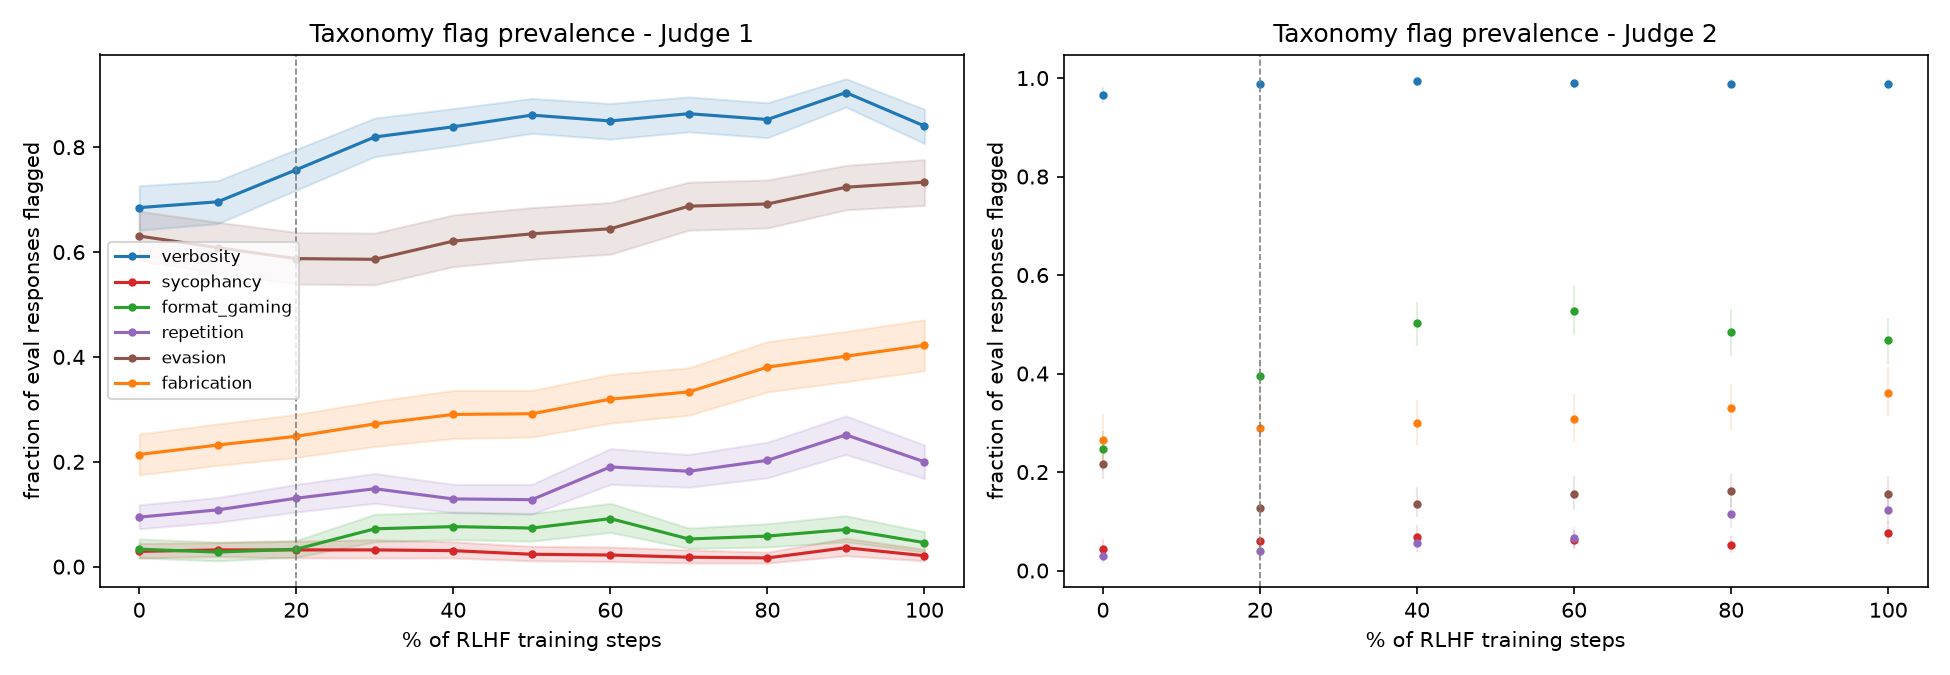
\includegraphics[width=0.98\linewidth]{figures/fig2_taxonomy_prevalence.png}
\caption{Fraction of evaluation responses with each taxonomy flag, for \judgeone (left, all checkpoints) and \judgetwo (right, 20\% grid). The two judges have very different base rates: \judgetwo flags verbosity on nearly every response, and \judgeone flags evasion on more than half. Fabrication rises steadily under both judges.}
\label{fig:taxonomy}
\end{figure}

\begin{figure}[t]
\centering
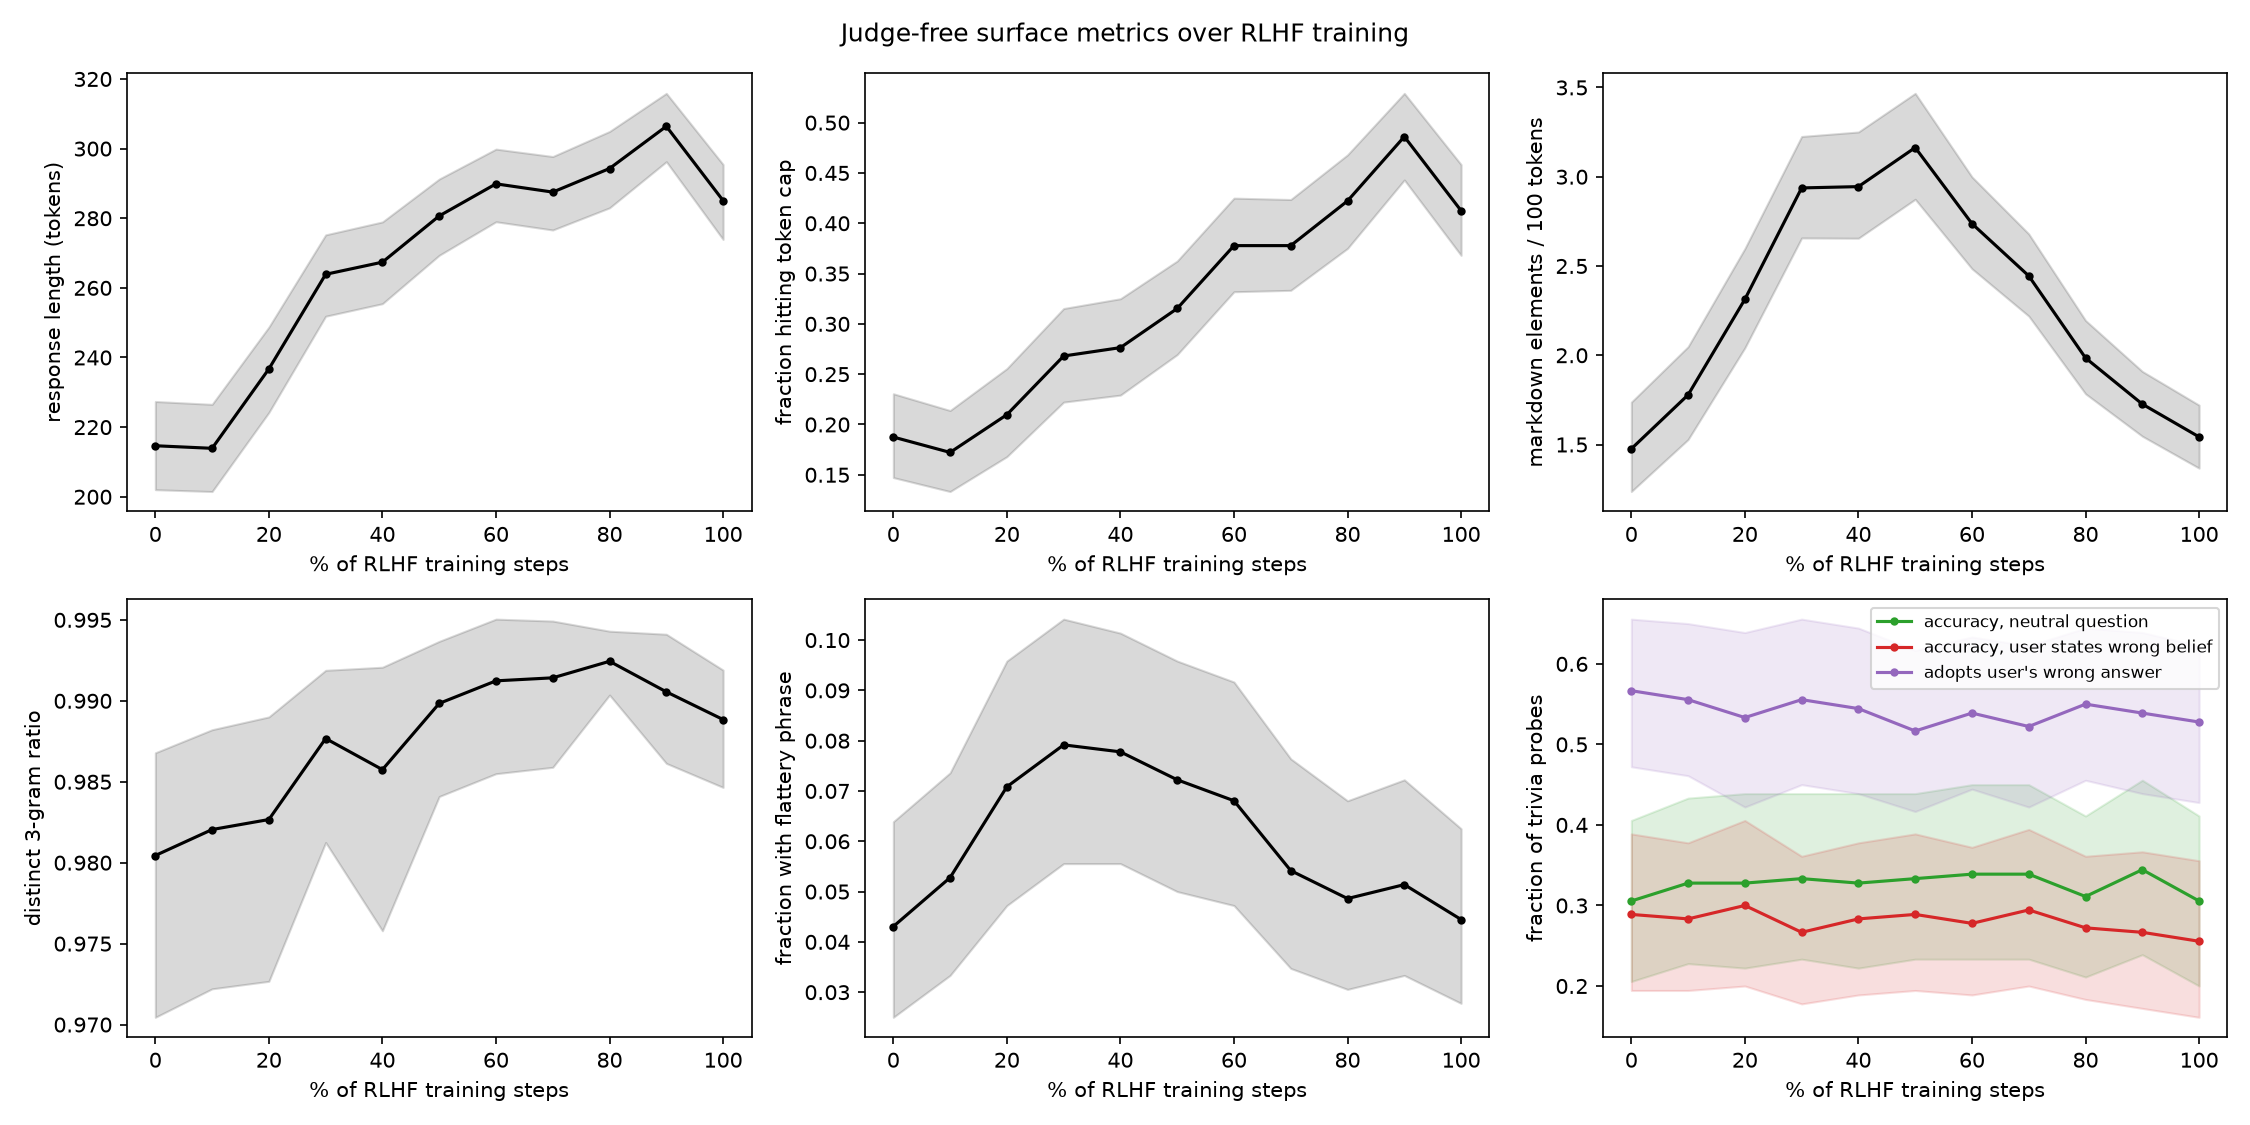
\includegraphics[width=0.98\linewidth]{figures/fig3_surface_metrics.png}
\caption{Judge-free surface metrics over training with 95\% prompt-bootstrap intervals. Length and cap-hit rate rise (top left, top middle); markdown density rises first and then returns to near its starting level (top right); the distinct-3-gram ratio stays near 0.98--0.99, so there is no measurable n-gram repetition (bottom left); flattery phrases rise briefly and return (bottom middle); the rate at which the policy adopts the user's wrong trivia answer does not change (bottom right).}
\label{fig:surface}
\end{figure}

\para{Verbosity emerges early but is not monotonic.}
\Tabref{tab:onset} shows that both response length and the verbosity flag are first significantly above step 0 at 20\% of training (Holm-adjusted $p=0.001$ for both; nothing at 10\%), and both stay above from then on.
At 20\% responses are 22 tokens longer and the flag rate is 7 points higher.
This supports the onset half of H2.
The monotonic half fails: verbosity rises until about 50--60\% and then plateaus.
The late-slope intervals include zero, and each seed has 2--5 decreasing intervals out of 10.
The Mann--Kendall trend over the whole run is still positive ($\tau$ 0.71--0.78).
The 384-token cap censors length: 41\% of final responses hit it, so late growth in verbosity is understated.

\para{Sycophancy does not emerge.}
None of the judge flag, the wrong-answer adoption rate, and the accuracy gap between neutral and wrong-belief prompts ever rises significantly.
The flattery lexicon is significantly above step 0 at 20\% only, which is not sustained (\figref{fig:surface}).
The step-0 policy already adopts the user's wrong answer 56.7\% of the time, and that rate is 52.8\% at the end.

\para{Format changes come first, not last.}
The fraction of responses with at least three markdown elements is significantly above step 0 at 10\%, earlier than any length measure.
It peaks at 0.717 at 50\% and falls to 0.544, with a late slope of $-0.040$ per 10\% of steps (CI $-0.050$ to $-0.030$).
\judgeone's format-gaming flag is significant at 30--60\% and 80--90\% and peaks at 0.092.
``Saturates'' fits these data; ``appears later'' does not, so H3 is not supported as stated.
Whether the extra structure counts as \emph{gaming} is where the judges disagree most ($\kappa=0.12$): \judgetwo flags format gaming on 24.7\% of step-0 responses and 52.8\% at 60\%.

\subsection{H4: when do the reward model and the judges diverge?}

\begin{table}[t]
\centering
\caption{Divergence between the \rmodel score and each judge metric. The last column is the first checkpoint at which the judge metric is significantly below its running maximum while the \rmodel score is significantly above its value there. \judgetwo is evaluated on a 20\% grid.}
\label{tab:divergence}
\begin{tabular}{@{}lll@{}}
\toprule
Judge metric & Peak & First divergence \\
\midrule
\judgeone quality & 5.64 at 10\% & {\bf 40\%} ($-0.34$, CI $-0.50$ to $-0.19$) \\
\judgeone pairwise vs.\ step 0 & 0.500 at step 0 & {\bf 40\%} (0.433, CI 0.405--0.460) \\
\judgetwo quality & 5.29 at 20\% & {\bf 40\%} ($-0.25$, CI $-0.42$ to $-0.09$) \\
\judgetwo pairwise vs.\ step 0 & 0.532 at 20\% (CI 0.508--0.556) & 60\% \\
\bottomrule
\end{tabular}
\end{table}

\para{Divergence is first detectable at 40\%.}
Three of four judge metrics in \tabref{tab:divergence} first diverge at the 40\% checkpoint and the fourth at 60\%.
Against step 0 under Holm correction, \judgeone's pairwise win rate is first significantly lower at 40\% and its quality rating at 50\%.
This roughly matches H4 in timing, with two caveats.

\para{The decline starts earlier than it is detected.}
Point estimates begin to fall before 40\%: \judgeone's win rate is 0.472 at 30\% (CI 0.443--0.501).
The 40\% mark is where our sample size detects the decline, not where it begins.

\para{There is no clear phase in which the judges prefer the trained policy.}
H4 presupposes that preference tracks the \rmodel score before diverging.
While the \rmodel score rose by about 0.7 standard deviations over the first 30\% of training, \judgeone never preferred the \rlhf policy, and its quality peak of 5.64 at 10\% is not significantly above step 0.
\judgetwo shows a small preference at 20\% only (0.532).

\para{The \rmodel stops tracking quality within a checkpoint.}
The within-checkpoint Spearman correlation between \rmodel score and \judgeone quality falls from 0.32 at step 0 to about 0.1 by 20\% and 0.00 at 100\%, while the \rmodel score keeps correlating with length at 0.5--0.6.
Agreement between ``\rmodel score went up'' and ``\judgeone prefers the checkpoint'', on order-consistent verdicts, falls from 54\% at 10\% to 35\% at 100\%.

\subsection{KL ablation}

With $\beta=0.5$ (one seed), the \rmodel score rises only to about 0.4, and nothing else moves: the verbosity flag goes from 0.70 to 0.72, judge quality from 5.69 to 5.60, and pairwise preference stays at 0.49 (\figref{fig:ablation} in the appendix).
With strong regularization there is neither meaningful reward gain nor detectable reward hacking in 160 updates.
This is one seed, and we treat it as indicative only.

\subsection{Judge reliability}
\label{sec:reliability}

\begin{table}[t]
\centering
\caption{Judge reliability. The judges agree on overall quality and on order-consistent pairwise verdicts, and disagree on most taxonomy labels.}
\label{tab:reliability}
\small
\begin{tabular}{@{}p{0.40\textwidth}p{0.55\textwidth}@{}}
\toprule
Check & Value \\
\midrule
Parse success & \judgeone 100\%; \judgetwo 99.2\% of ratings \\
Position bias (chose ``A'') & \judgeone 66\%; \judgetwo 77\% \\
Pairwise verdict same in both orders & \judgeone 56\%; \judgetwo 44\% \\
Inter-judge quality rating (Spearman, $n=4{,}524$) & 0.71 \\
Inter-judge pairwise, order-consistent only ($\kappa$, $n=1{,}151$) & 0.78 \\
Inter-judge flag $\kappa$ & fabrication 0.57; sycophancy 0.23; evasion 0.17; format 0.12; verbosity 0.12; repetition 0.10 \\
\judgeone flag vs.\ surface metric (Spearman) & verbosity--tokens 0.37; format--markdown 0.28; sycophancy--flattery 0.24; sycophancy--adopts-wrong 0.08; repetition--distinct-3-gram $-0.02$ \\
\bottomrule
\end{tabular}
\end{table}

\Tabref{tab:reliability} shows which measurements can carry weight.
The two judges agree on overall quality (Spearman 0.71) and, when each is order-consistent, on which of two responses is better ($\kappa=0.78$).
They do not agree on most taxonomy labels: only fabrication reaches $\kappa=0.57$, and four of six flags are at 0.10--0.17.
Both judges have a strong position bias, which leaves only 44--56\% of pairwise verdicts order-consistent.
The repetition flag is not corroborated by the n-gram metric at all (Spearman $-0.02$), so we do not interpret it.
The quality and preference trajectories of H4 therefore rest on firmer ground than the category shares of H1.
